\subsection{Functional Areas}
\label{sec:functional-areas}

Before describing how the application's functional requirements are structured within the system architecture, it is necessary to clarify the distinction between an application and a system. An application is a software program that performs specific tasks, whereas a system is a collection of interacting components, among which the application is considered one element.

Within this system, functional requirements are organized into functional areas based on shared purpose or behavior. Each functional area groups related use cases performed by a specific actor. To illustrate the structure of these areas, a dedicated UML Use Case diagram is provided for each one.

In this context, actors represent the application's end users. Two types of actors are identified: Users and Administrators (labeled as “Admin” in the diagrams). The user category includes both ordinary employees and administrators. Administrators, in addition to general user capabilities, possess further permissions to review and manage the expense reports submitted by employees under their supervision.

To illustrate how these use cases are implemented, this section provides a detailed technical description for three critical and representative use cases: user authentication, expense registration via file upload, and report approval. These specific examples have been carefully selected because they best demonstrate the system's core functionalities, security mechanisms, asynchronous processing architecture, and multi-role interactions.

The complete and exhaustive technical description to all use cases diagrammed in this section, including their respective actors, triggers, pre/postconditions, and detailed event flows, is available for comprehensive review in Appendix~\ref{appendix:use_case_specifications}: Detailed Use Case Specifications.

\subsubsection{Account Management}
\label{sec:account-management}

This functional area covers all use cases related to user accounts. Since the application's core functionality is expense management, user login is the only required action. The resulting use case diagram is presented in Figure \ref{fig:account-management-use-case-diagram}.

\begin{figure}[H]
    \centering
    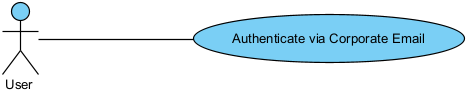
\includegraphics[width=0.6\textwidth]{Images/accountmanagement.png}
    \caption[Account management use case diagram]
    {Account management use case diagram. [Own creation]}
    \label{fig:account-management-use-case-diagram}
\end{figure}

\vspace{1cm}

\textbf{Use Case: Authenticate via Corporate Email}

\textbf{Primary Actor:} User

\textbf{Trigger:} The user attempts to access the application URL.

\textbf{Preconditions:} None.

\textbf{Postconditions:} The user is authenticated and redirected to the home page with role-specific access.

\vspace{0.5cm}

\textbf{Main Success Scenario:}

\begin{enumerate}  [leftmargin=0.75cm, noitemsep]
    \item The user navigates to the web application and initiates the login process.
    \item The system displays the login interface.
    \item The user enters their account credentials.
    \item The system authenticates the credentials successfully.
    \item The system verifies that the email belongs to the authorized corporate domain.
    \item The system assigns the corresponding role to the user and redirects them to the home page, displaying the available functionalities according to the user's assigned role.
\end{enumerate}

\vspace{0.3cm}

\textbf{Extensions:}

\begin{itemize} [label={}, leftmargin=0.75cm, noitemsep]
    \item \textbf{2a. Server Connection Error:}
    \begin{itemize} [label={}, leftmargin=0.75cm, noitemsep]
        \item 2a1. The system cannot connect to the server and cannot display the login interface.
    \end{itemize}

    \item \textbf{4a. Authentication Failed (Invalid Credentials):}
    \begin{itemize} [label={}, leftmargin=0.75cm, noitemsep]
        \item 4a1. The system displays an invalid credentials error message (``Invalid email'' or ``Invalid password'').
        \item 4a2. The user remains on the login page and returns to step 3 until valid credentials are provided.
    \end{itemize}

    \item \textbf{5a. Unauthorized Domain:}
    \begin{itemize}  [label={}, leftmargin=0.75cm, noitemsep]
        \item 5a1. The system detects that the authenticated account does not belong to the authorized corporate domain.
        \item 5a2. The system denies access and notifies the user.
    \end{itemize}
\end{itemize}



\subsubsection{Expense Management}
\label{sec:expense-management}

This functional area encompasses all features related to expense management. It includes functionalities such as uploading, editing, and deleting expenses, as well as obtaining AI-extracted data and assigning expenses to either a new or an existing report. All these actions are accessible within the Expenses List page view, as shown in Figure \ref{fig:expense-management-use-case-diagram}.

\begin{figure}[H]
    \centering
    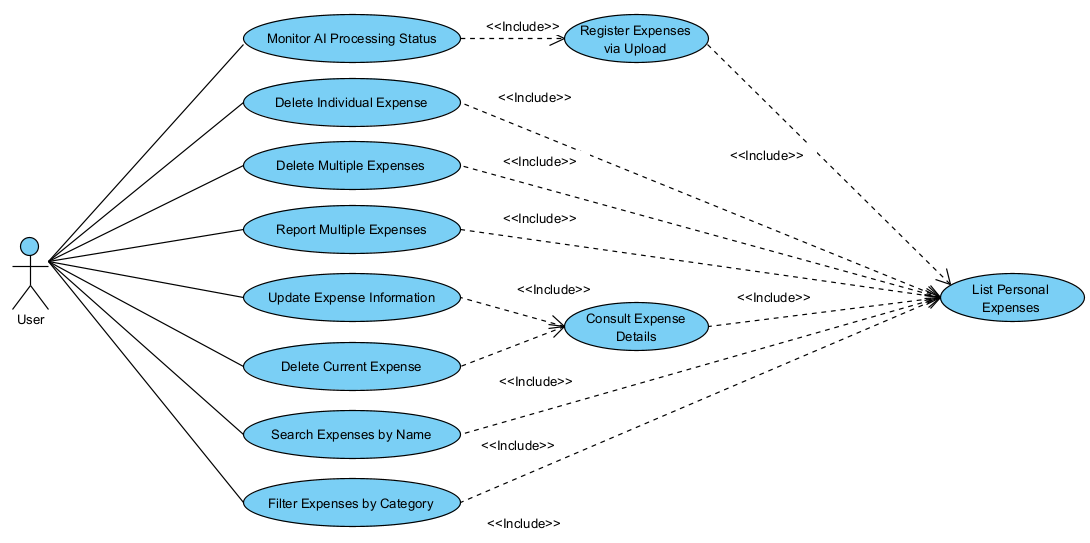
\includegraphics[width=\textwidth]{Images/expensemanagement.png}
    \caption[Expense management use case diagram]
    {Expense management use case diagram. [Own creation]}
    \label{fig:expense-management-use-case-diagram}
\end{figure}

\textbf{Use Case: Register Expenses via Upload}

\textbf{Primary Actor:} User

\textbf{Trigger:} The user uploads or drops one or more receipts.

\textbf{Preconditions:} The user is successfully authenticated and viewing the Expenses page.

\textbf{Postconditions:} The new expenses are successfully registered and added to the AI processing queue.

\vspace{0.5cm}

\textbf{Main Success Scenario:}

\begin{enumerate}[leftmargin=0.75cm, noitemsep]
    \item The user uploads or drops one or more receipts.
    \item The system registers new expense records, associates them with the authenticated user, and queues them for automated data extraction.
    \item The system updates the expense list to include the recently uploaded items.
\end{enumerate}

\vspace{0.3cm}

\textbf{Extensions:}

\begin{itemize}[label={}, leftmargin=0.75cm, noitemsep]
    \item \textbf{2a. Invalid File Format:}
    \begin{itemize}[label={}, leftmargin=0.75cm, noitemsep]
        \item 2a1. The system detects that the uploaded file format is not supported (non-image or non-PDF).
        \item 2a2. The system rejects the upload and keeps the user on the current page without registering any expense.
    \end{itemize}

    \item \textbf{2b. Database Connection Error:}
    \begin{itemize}[label={}, leftmargin=0.75cm, noitemsep]
        \item 2b1. The system is unable to register the expense records due to a database connection failure.
        \item 2b2. The system notifies the user of the error and no expenses are registered.
    \end{itemize}
\end{itemize}
\subsubsection{Report Management}
\label{sec:report-management}

This functional area groups all the operations related to report management. In this application, a report serves as a container for a set of expenses prepared for submission. Once a report has been reviewed and finalized, it is submitted to the appropriate reviewer. 

Core functionalities within this area include creating, modifying, deleting, and submitting reports. Additionally, expenses can be easily attached or detached to a report, and any assigned expenses can be updated while preserving data consistency. The use case diagram for this functional area is shown in Figure \ref{fig:report-management-use-case-diagram}.


\begin{figure}[H]
    \centering
    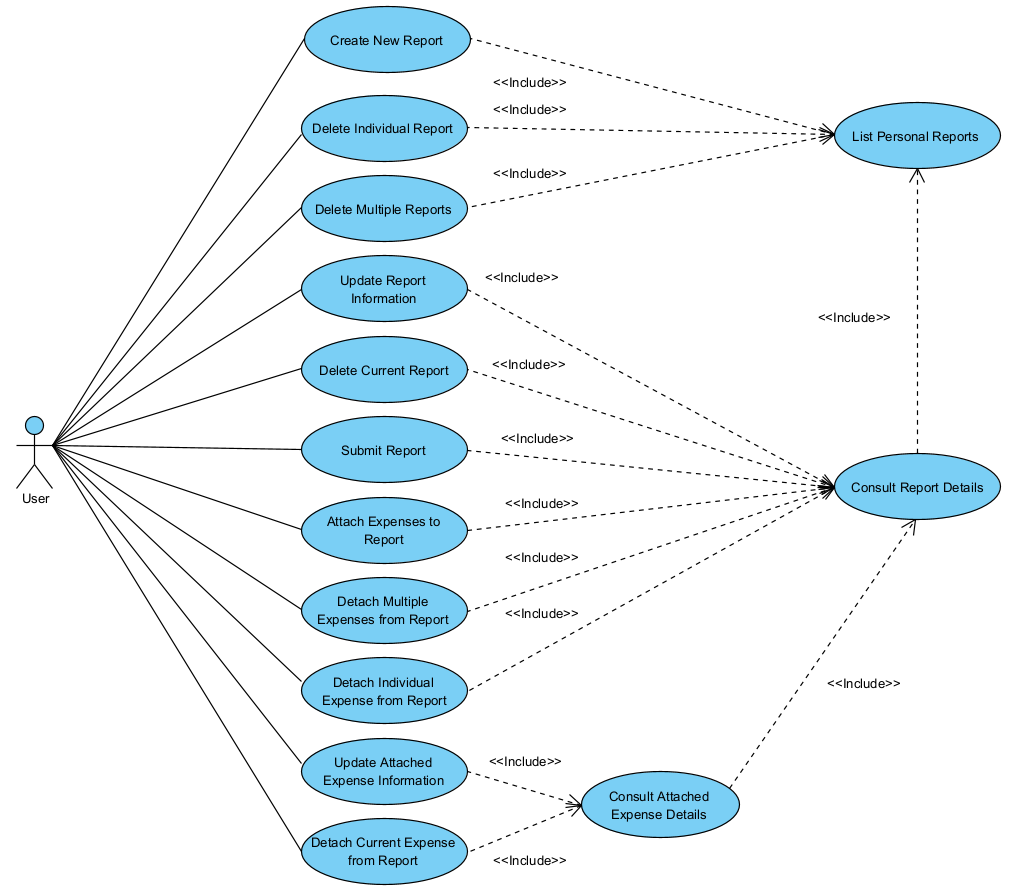
\includegraphics[width=\textwidth]{Images/reportmanagement.png}
    \caption[Report management use case diagram]
    {Report management use case diagram. [Own creation]}
    \label{fig:report-management-use-case-diagram}
\end{figure}
\subsubsection{Submitted Report Management}
\label{sec:submitted-report-management}

This functional area allows users to monitor the real-time status of their reports. It enables them to determine whether submitted expenses have been reviewed and approved or rejected by a supervisor. As submitted reports are no longer editable, user interaction is limited to viewing report details and the associated expenses. This functional area is accessible to all users. Figure \ref{fig:submitted-report-management-use-case-diagram} depicts the corresponding use case diagram.

\begin{figure}[H]
    \centering
    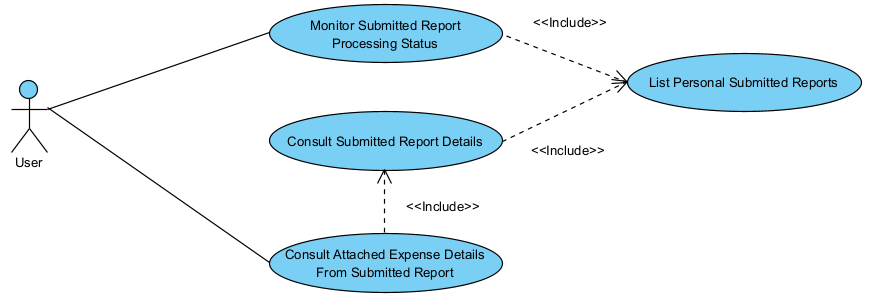
\includegraphics[width=\textwidth]{Images/submittedreportmanagement.png}
    \caption[Submitted report management use case diagram]
    {Submitted report management use case diagram. [Own creation]}
    \label{fig:submitted-report-management-use-case-diagram}
\end{figure}
\subsubsection{Pending Review Report Management}
\label{sec:pending-review-report-management}

Unlike the previously described functional areas, this area is accessible only to administrative users, who are responsible for supervising ordinary employees. Within this area, administrators can view all pending reports and their associated expenses, and decide whether to approve or reject them. All use cases are represented in the diagram shown in Figure \ref{fig:pending-review-report-management-use-case-diagram}.

\begin{figure}[H]
    \centering
    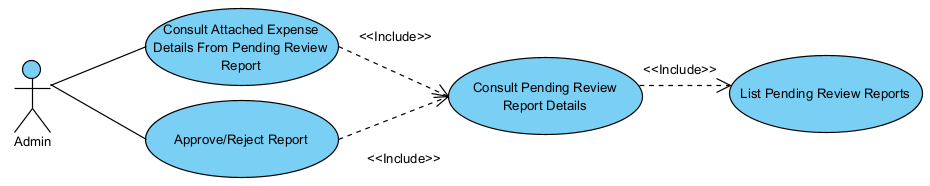
\includegraphics[width=\textwidth]{Images/pendingreviewreportmanagement.png}
    \caption[Pending review report management use case diagram]
    {Pending review report management use case diagram. [Own creation]}
    \label{fig:pending-review-report-management-use-case-diagram}
\end{figure}

\textbf{Use Case: Approve/Reject Report}

\textbf{Primary Actor:} Administrator

\textbf{Trigger:} The administrator approves or rejects a report pending review.

\textbf{Preconditions:} The administrator is authenticated, and the system displays the report metadata along with a list of associated expenses.

\textbf{Postconditions:} The system updates the report status according to the administrator's decision.

\vspace{0.5cm}

\textbf{Main Success Scenario:}

\begin{enumerate}[leftmargin=0.75cm, noitemsep]
    \item The administrator approves or rejects the currently displayed report.
    \item The system updates the report status accordingly and notifies the report owner of the review.
\end{enumerate}

\vspace{0.3cm}

\textbf{Extensions:}

\begin{itemize}[label={}, leftmargin=0.75cm, noitemsep]
    \item \textbf{2a. Report Review Error:}
    \begin{itemize}[label={}, leftmargin=0.75cm, noitemsep]
        \item 2a1. An error occurs during the report review due to a database connection error or an internal error.
        \item 2a2. The system notifies the administrator of the error and keeps them on the current report details view.
    \end{itemize}
\end{itemize}
\subsubsection{Reviewed Report Management}
\label{sec:reviewed-report-management}

Finally, this functional area provides a record of all reports reviewed by the user and is therefore restricted to administrative users. Unlike the previous area, it only allows administrators to view reviewed reports and examine the details of each report and its associated expenses. Figure \ref{fig:reviewed-report-management-use-case-diagram} presents the use case diagram of this functional area.

\begin{figure}[H]
    \centering
    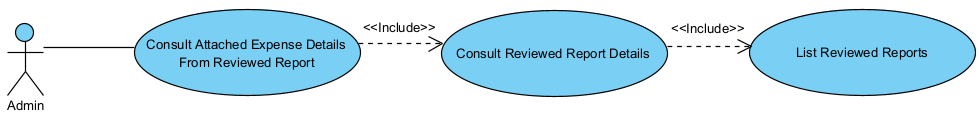
\includegraphics[width=\textwidth]{Images/reviewedreportmanagement.png}
    \caption[Reviewed report management use case diagram]
    {Reviewed report management use case diagram. [Own creation]}
    \label{fig:reviewed-report-management-use-case-diagram}
\end{figure}
